\documentclass{cmc}

\hypersetup{
    colorlinks=true,
    linkcolor=blue,
    filecolor=magenta,      
    urlcolor=red,
}
\urlstyle{same}

\begin{document}

\pagestyle{fancy}
\lhead{\textit{\textbf{Computational Motor Control, Spring 2018} \\
	Python exercise, Lab 0, NOT GRADED}} \rhead{Student \\ Names}

\section*{Student names: \ldots (please update)}

\textit{Instructions: This document contains the instructions to install and get
  familiarized with Python programming.  \textbf{This lab is not graded}. This
  file does not need to be submitted and is provided for your own benefit.}



\section{Course Organization}

This year all the exercises for the course will be distributed through GitLab.
GitLab is an online open source Git repository for maintaining and distributing
code between groups of people. The access to the exercises repository is public
and you can directly use your epfl credentials to login.  We
recommend you to use the features Git offers to collaborate with your partners and
maintain a history of your own work as well.  If you download the repository
without cloning,  then you will have to do it every week and you will end up
downloading all the previous files every time you do it. This report does not
contain a tutorial on how to use Git but you can find the references in section
\ref{sec:git_ref}. However, we will have short demo on how to use it during the
exercise hour.

The link to the \href{https://gitlab.epfl.ch/BioRobCMC/2018}{git repository}

\section{Python Setup}

This course expects you to complete the exercises using the standard Python
programming language.  There are many options to use Python. For those students
who are starting of new with Python, we strongly suggest to follow the following
installation steps of the Anaconda environment. For those familiar with Python,
you are free to use an environment of your choice but we still advise you to
set-up the Anaconda environment to ease the debugging process with the
assistants.

\subsection{Anaconda}
\label{subsec:anaconda}
Anaconda is an open source Python environment that sets up all the necessary
packages and softwares needed for scientific computing using Python.

Follow the \href{https://www.anaconda.com/download/}{link} to download Anaconda
distribution for your specific OS.

\textbf{Choose Python 2.7 for installation}.

Instructions for installation :

\begin{itemize}
\item \href{{https://docs.anaconda.com/anaconda/install/windows}}{Windows}
\item \href{https://docs.anaconda.com/anaconda/install/mac-os}{MacOS}
\item \href{https://docs.anaconda.com/anaconda/install/linux}{Linux}
\end{itemize}

To verify your installation :

\begin{itemize}
\item First open your terminal
  \begin{itemize}
  \item Windows: Open the Anaconda Prompt (Click Start, select Anaconda Prompt)
  \item MacOS: Open Launchpad, then open Terminal or iTerm.
  \item Linux–Ubuntu: Open the Dash by clicking the upper left Ubuntu icon, then
    type “terminal”.
  \end{itemize}
\item Enter a command such as \textit{conda list}. If Anaconda is installed and
  working, this will display a list of installed packages and their versions.
\end{itemize}

\subsection{Spyder}

Python programs can be written in several ways, it can be simply done on a
terminal by running \textit{python} or \textit{ipython}. While this method is
limited for simple programs, larger programs will be written using a text-editor
or an Integrated Development Environment (IDE).  Though it is not necessary to
have an IDE for programming in Python, having one will bring many features that
are useful while starting new. Once you have installed Anaconda successfully
using the section \ref{subsec:anaconda}, Spyder should be installed by default.

Spyder can be run by executing the command \textit{spyder} in a
terminal/anaconda-prompt.

Figure \ref{fig:spyder} shows the main windows when you first open Spyder. As
you may have noticed, the layout is similar to Matlab. Spyder has very good
documentation to get you started.  It is recommended to go through the steps to
get familiarized with the IDE.

\begin{figure}[h]
  \centering 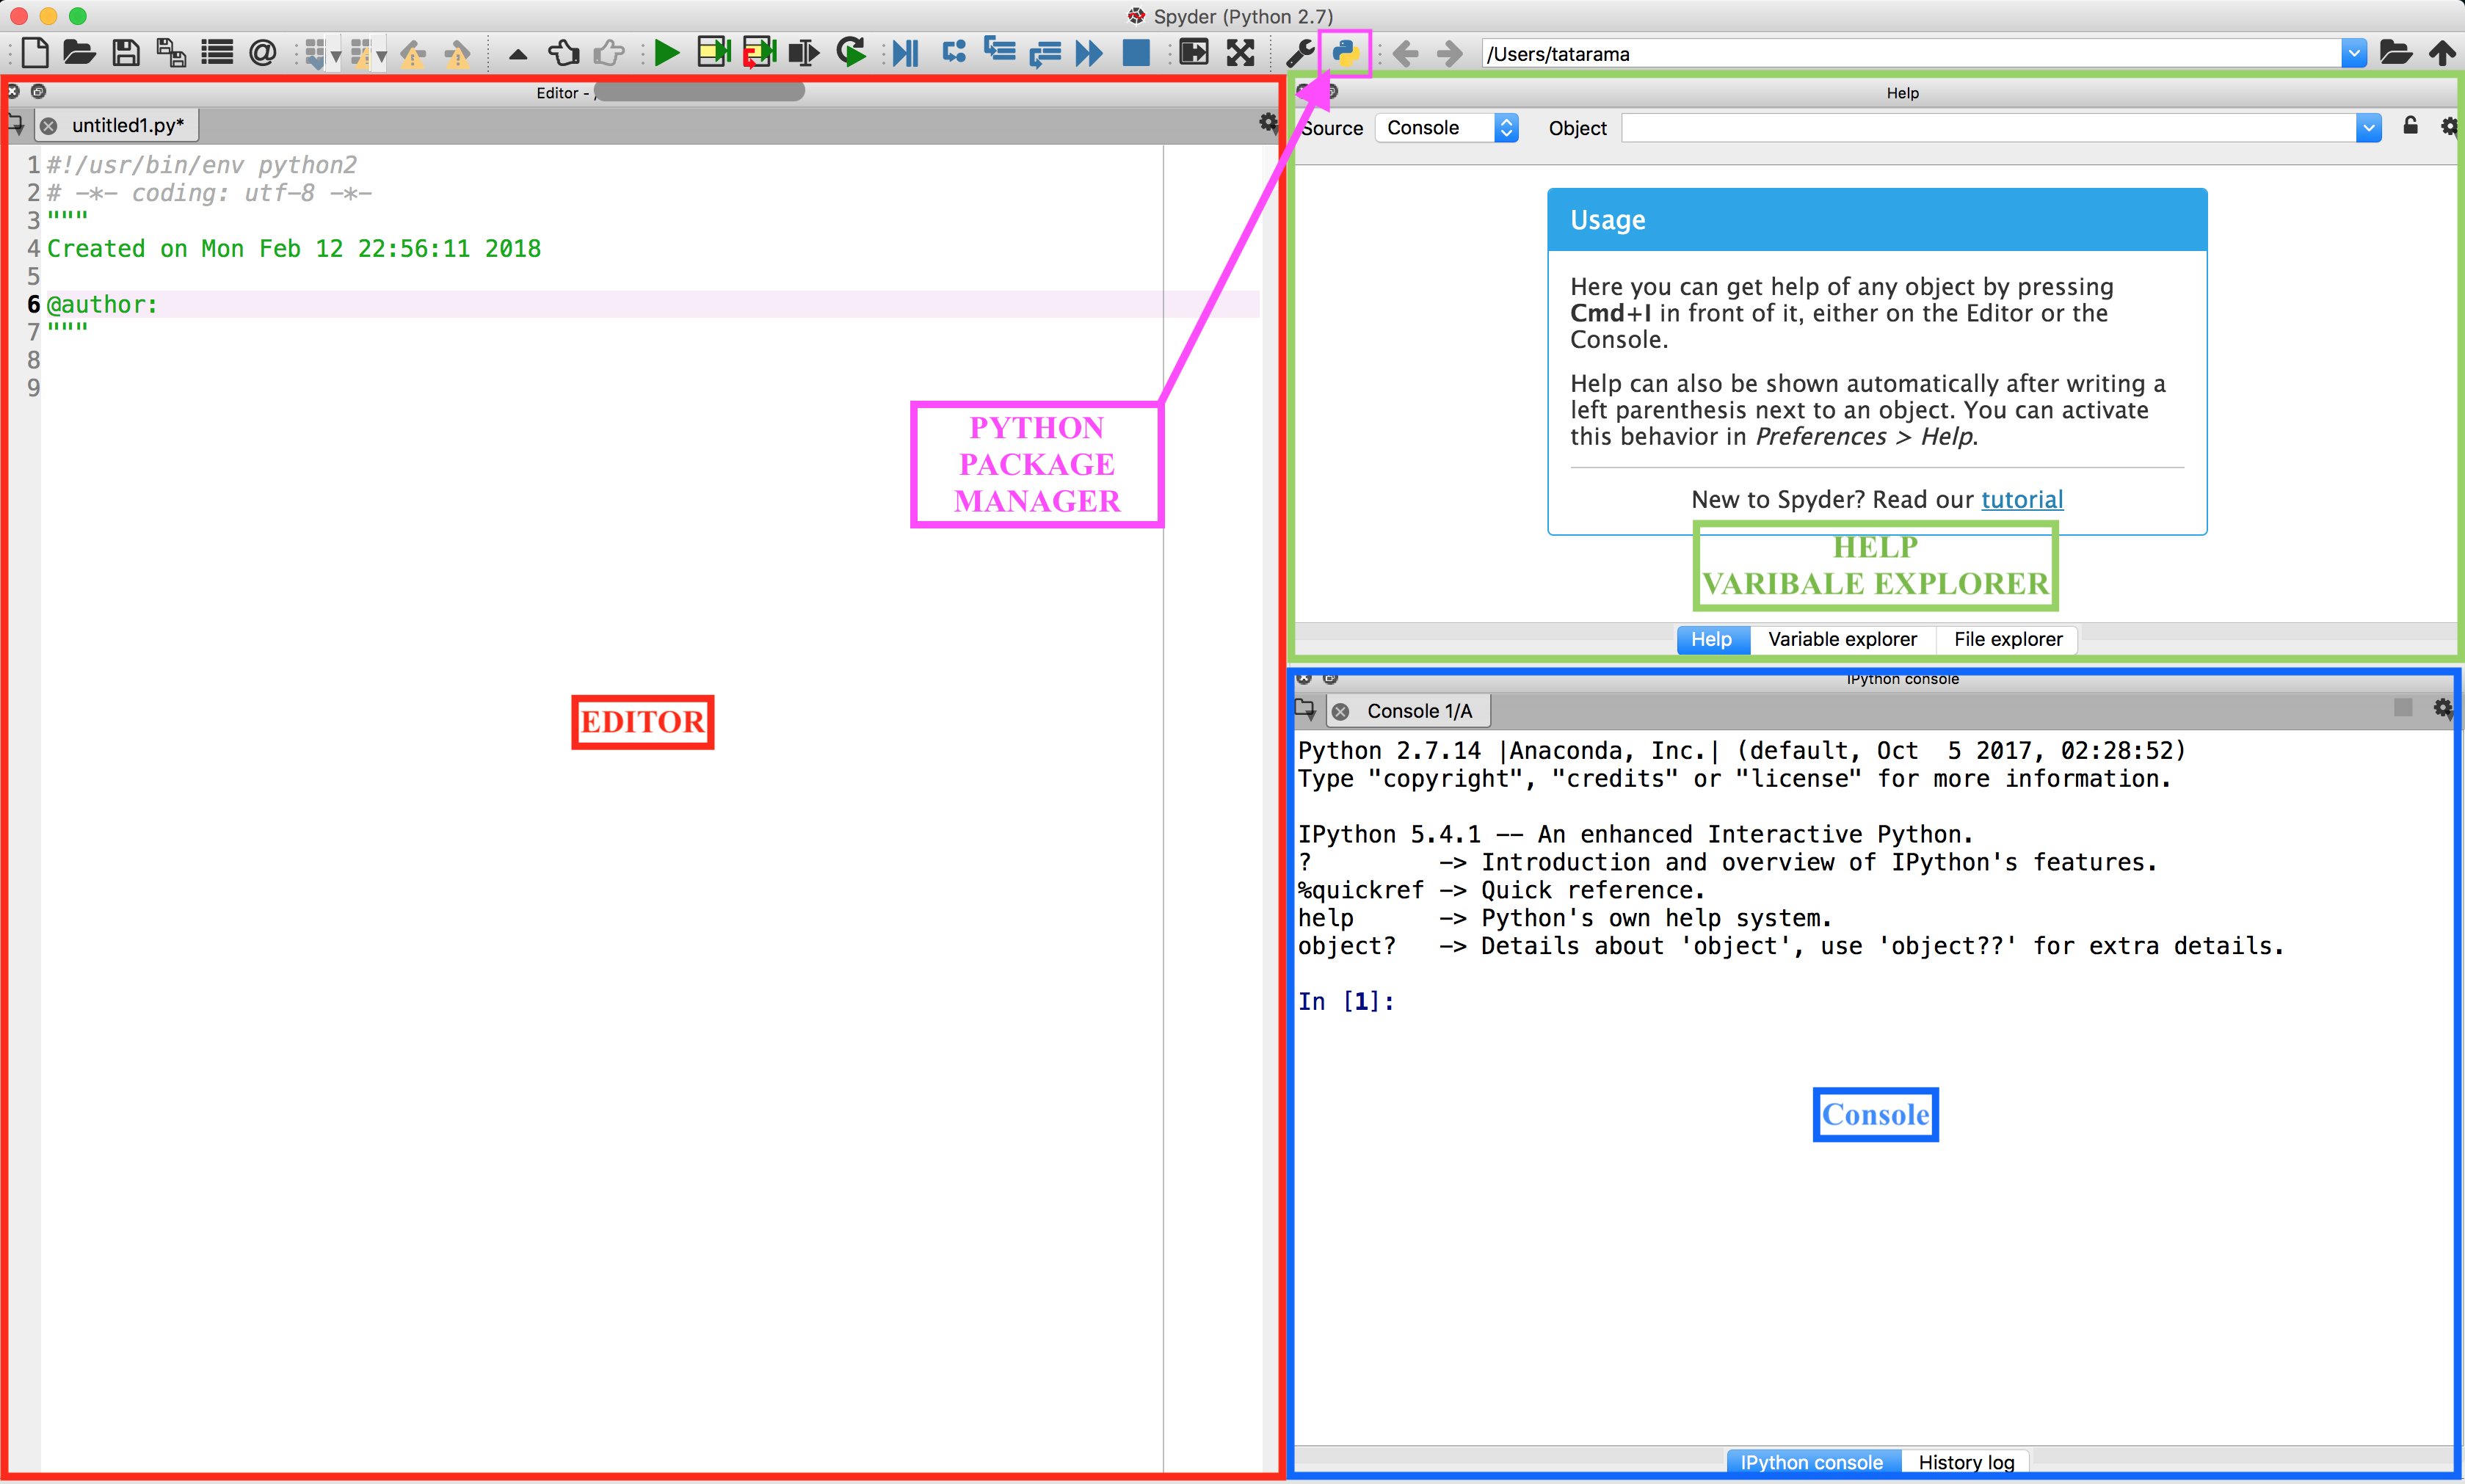
\includegraphics[width = \textwidth]{figures/Spyder.png}
  \caption{Spyder IDE overview}
  \label{fig:spyder}
\end{figure}

The three essential parts of the screen are outlined.

\begin{itemize}
\item \textbf{The console} (bottom right, marked in blue). You can work
  interactively here. Code run, either interactively or from the editor, will
  output any results here.  Error messages will be reported here. There are two
  types of console: a Python console, and an IPython console. Both will run
  Python code, but we recommend the IPython console as it offers better visuals
  for debugging and has additional features.
\item \textbf{The editor} (left, marked in red). You can write code to be saved
  to file or run here. This will suggest problems with syntax and has features
  to help debug and give additional information.
\item \textbf{The inspector} (top right, marked in green). The Object inspector
  can display detailed help on specific objects (or functions, or...), and the
  Variable inspector can display detailed information on the variables that are
  currently defined. Extremely useful when debugging.
\item \textbf{Python Package Manager} (top toolbar, marked in pink) Use this
  menu to add new paths to the default python package paths. (NOTE : The symbol
  may look slightly different on your machine from the one shown in this report)
\end{itemize}

For an in depth tutorial of Spyder follow the
\href{http://www.southampton.ac.uk/~fangohr/blog/spyder-the-python-ide.html#first-steps-with-spyder}{link}.

Before you begin with the programming, there is one more important
step. Assuming that you have either downloaded or cloned the exercises
repository from GitLab, we now have to add some python packages that will be
used through out this course. To do this,
\begin{itemize}
\item Open the Python Package manager window (The icon marked in pink in the
  figure \ref{fig:spyder})
\item Click on Add Path
\item Navigate to the downloaded exercise repository and add the
  \textbf{PythonPackages} folder
\item Close and re-open Spyder
\end{itemize}

\section{Programming with Python}

After successfully completing the installation steps in the previous section,
you can now get started with programming using Python.  Python is not just a
computational tool but a very powerful programming language. This means having
to learn a few more extra concepts to get your job done.  There are a ton of
references available online for those who are interested in learning Python in
depth. We will try to provide the necessary references to help with the concepts
that are useful during the course as and when needed.

\subsection{Basic Python Concepts}

In this section we will quickly go over the list of topics given below. You can open and run the individual files marked with the same topic name using Spyder.
We suggest you to go through each section individually and spend time exploring each of the concepts by making changes to the code and observing the outputs.

\begin{enumerate}
        \item HelloWorld
	\item Imports
	\item Data Types
	\item Math
	\item Conditional Statements
	\item Data Containers : Lists, Tuples and Dictionaries
	\item Functions
	\item Loops
	\item Numpy
	\item Matplotlib
\end{enumerate}

While you are executing each of the small exercises, try to learn how to use different features of Spyder. Especially the help and debugging feature.
When you are unsure of any command, use the help service either the one built into Python or Spyder.
After familiarizing yourself with the above concepts try to solve the following python exercises.

\subsection{Exercise 1}
\textbf{Check if the following matrix M is a magic square or not?}

\textit{\textbf{Hint : } A magic square is a square matrix which contains distinct integers and whose sum along any of its individual rows or columns or diagonal is a constant.
The constant is called as a magic constant or magic sum or magic square}

\begin{equation*}
  \label{eq:1}
  M = 
  \begin{bmatrix}
    16 & 3  & 2  & 13 \\
    5  & 10 & 11 & 8  \\
    9  & 6  & 7  & 12 \\
    4 & 15 & 14 & 1
  \end{bmatrix}
\end{equation*}

\textit{\textbf{Further Step : } Try if you can generalize your script to have a
  function to check any arbitrary matrix if it is a magic square or not.  Import
  the function as a module in another script and use it to check the matrix M}

\subsection{Exercise 2 - Plotting a function}

\textit{Plot the following function $f(x)$ over an interval [0, 2] with proper
  labels and title}

\begin{equation*}
  \label{eq:3}
  f(x) = sin(x - 2)e^{-x^2}
\end{equation*}

\newpage
\section{References}
\label{sec:references}

\subsection{Python}
\label{sec:python_ref}
\begin{itemize}
\item \href{http://mathesaurus.sourceforge.net/matlab-numpy.html}{NumPy for
    MATLAB users}
\item \href{https://python.swaroopch.com}{A byte of python}
\item \href{http://nbviewer.jupyter.org/gist/rpmuller/5920182}{A Crash Course in
    Python for Scientists}
\item The official \href{https://docs.python.org/2/}{Python documentation}
  should be your first stop when looking for information
\item \href{http://numpy.scipy.org/}{numpy}
\item \href{http://www.scipy.org/}{scipy}
\item \href{http://matplotlib.sourceforge.net/}{matplotlib}
\end{itemize}

\subsection{Git}
\label{sec:git_ref}
\begin{itemize}
\item \href{https://try.github.io/levels/1/challenges/1}{Try Git!}
\item \href{https://marklodato.github.io/visual-git-guide/index-en.html}{A
    Visual Git Reference}
\end{itemize}

\end{document}
%%% Local Variables:
%%% mode: latex
%%% TeX-master: t
%%% End:

%  LocalWords:  iTerm
